
\documentclass{ppgeesa}

%%%%%%%%%%%%%%%%%%%%%%%%%%%%%%%%%%%%%%%%%%%%%%%%%%%%%%%%%%%%%%%%%%%%%%%%%%%%%%%%%%%%%%%%%%%%%%%%%%%%%%%%%%%%%%%%%

\usepackage[latin1]{inputenc}
\usepackage{graphicx}
\usepackage{hyperref}
\usepackage{tikz}
\usepackage{amsmath}
\usepackage{listings}

\lstset{ %
language=Matlab,                % choose the language of the code
basicstyle=\footnotesize,       % the size of the fonts that are used for the code
numbers=none,                   % where to put the line-numbers
numberstyle=\footnotesize,      % the size of the fonts that are used for the line-numbers
stepnumber=2,                   % the step between two line-numbers. If it's 1 each line 
                                % will be numbered
numbersep=5pt,                  % how far the line-numbers are from the code
backgroundcolor=\color{white},  % choose the background color. You must add \usepackage{color}
showspaces=false,               % show spaces adding particular underscores
showstringspaces=false,         % underline spaces within strings
showtabs=false,                 % show tabs within strings adding particular underscores
frame=false,	                % adds a frame around the code
tabsize=2,		                % sets default tabsize to 2 spaces
captionpos=b,                   % sets the caption-position to bottom
breaklines=true,                % sets automatic line breaking
breakatwhitespace=true,         % sets if automatic breaks should only happen at whitespace
title=\lstname,                 % show the filename of files included with \lstinputlisting;
                                % also try caption instead of title
escapeinside={\%*}{*)}         % if you want to add a comment within your code
%morekeywords={*,...}            % if you want to add more keywords to the set
}
\lstset{caption=Descriptive Caption Text,label=DescriptiveLabel}

\hypersetup{
	colorlinks,
	debug=true,
	linkcolor=black,  %%% cor do tableofcontents, \ref, \footnote, etc
	citecolor=red,  %%% cor do \cite
	urlcolor=blue,   %%% cor do \url e \href
	bookmarksopen=true,
	pdftitle={Modelagem e identifica��o de sistemas},
	pdfauthor={Tassiano Neuhaus},
	pdfsubject={M�todos param�tricos de identifica��o},
	pdfkeywords={Identifica��o de sistemas}
	%pdfpagemode=FullScreen
}

%%%%%%%%%%%%%%%%%%%%%%%%%%%%%%%%%%%%%%%%%%%%%%%%%%%%%%%%%%%%%%%%%%%%%%%%%%%%%%%%%%%%%%%%%%%%%%%%%%%%%%%%%%%%%%%%%


\begin{document}

\title{M�todos param�tricos de identifica��o de sistemas - Trabalho 3}

\author{Tassiano Neuhaus\\
{\small Universidade Federal do Rio Grande do Sul - Departamento de Engenharia El�trica\\Av. Osvaldo Aranha, 103 - Bairro Bom Fim CEP: 90035-190 - Porto Alegre - RS - Brasil}\\
}%\thanks{Tassiano Neuhaus, tassianors@gmail.com, tel +55-51-91760154}}

\maketitle
\thispagestyle{empty}\pagestyle{empty}

\begin{abstract}
Este trabalho tem o objetivo de demonstrar tr�s diferentes m�todos para identificac�o de um 
sistema. 
\end{abstract}

\begin{IEEEkeywords}
Identifica��o de sistemas lineares, m�todos param�tricos.
\end{IEEEkeywords}

%===============================================================================
\section{Introdu��o}

Neste trabalho ser� apresentado o projeto de controladores denominados Robustos. Para 
tanto ser� apresentado o conceito de um controlador Robusto. A fim de modelar um
sistema sujeito a incertezas ser� apresentado alguns m�todos para que sua modelagem
matem�tica seja poss�vel. 

Para tornar o estudo mais claro ser� utilizado um sistema f�sico onde estar� sujeito a
perturba��es e/ou incertezas. Sobre este sistema ser� feito a modelagem seguindo cada um
dos processos e com estes modelos ser� efetuado uma simula��o. 

Esta simula��o ser� baseada no projeto de uma realimenta��o de estados com o intuito de
satisfazer a minimiza��o da norma $H2$ e $H_{\infty}$.

O sistema utilizado � apresentado no sistema de equa��es de estado descrito em (\ref{eq:intro_sis}).

\begin{equation}
\begin{matrix}
A=\begin{bmatrix}
0 & 1\\ 
-ba &a+b 
\end{bmatrix} &
B=\begin{bmatrix}
0\\ 
k
\end{bmatrix} 
\end{matrix}
\label{eq:intro_sis}
\end{equation}

Este sistema possui a fun��o de transfer�ncia apresentado em (\ref{eq:intro_transf}).

\begin{equation}
G(s)=\frac{k}{(s-a)(s-b)}
\label{eq:intro_transf}
\end{equation}

Os par�metros $a, b, k$ est�o sujeitos as varia��es apresentadas em (\ref{eq:intro_limit}).

\begin{equation}
\begin{matrix}
b= & -0.012725 & \\ 
k= & [k_1 \; k_2] =& [-0.4649.10^{-4} \; -0.7449.10^{-4}]\\ 
a= & [a_1 \; a_2] =& [-0.25 \; -2]
\end{matrix}
\label{eq:intro_limit}
\end{equation}


\section{Identifica��o}
\label{sec:identification}
%===============================================================================

O sistema em estudo � composto por uma fonte de tens�o alimentado um resistor. O prop�sito
deste trabalho � apresentar tr�s diferentes m�todos para identifica��o da resist�ncia do
resistor do sistema.

Para identifica��o do sistema foram feitos dois conjuntos de medidas de tens�o e corrente
sobre o resistor que s�o apresentados na Tabela (\ref{tab:data}).

\begin{table}[htbp]
  \begin{center}
	\caption{Medidas sobre o sistema}
	\label{tab:data}
	\begin{small}
	  \begin{tabular}{cllllll}
		\hline
		Medida	&  V1 & V2 & V3 & I1 & I2 & I3 \\
		t		&    & y(t)[V] &  &    & u(t)[mA] & \\
		\hline
		1	& 1.45	& 1.28	 & 1.28 & 0.94	& 0.81	& 0.82 \\
		2	& 2.58	& 2.14	 & 1.71 & 1.6	& 1.2	& 1.1 \\
		3	& 3.08	& 2.71	 & 2.21 & 2.02	& 1.68	& 1.25 \\
		4	& 3.54	& 3.51	 & 3.02 & 2.3	& 2.28	& 1.94 \\
		5	& 4.01	& 4.49	 & 3.64 & 2.63	& 2.81	& 2.22 \\
		6	& 4.57	& 5.05	 & 4.12 & 3.01	& 3.27	& 2.68 \\
		7	& 5.21	& 6.05	 & 4.82 & 3.42	& 3.9	& 3.12 \\
		8	& 6.21	& 6.72	 & 5.25 & 4.09	& 4.22	& 3.42 \\
		9	& 7.09	& 7.45	 & 6.11 & 4.51	& 4.81	& 4 \\
		10	& 7.71	& 8.13	 & 6.88 & 4.91	& 5.3	& 4.55 \\
		11	& 8.36	& 8.9	 & 7.6  & 5.49	& 5.78	& 5.05 \\
		12	& 9.06	& 9.73	 & 8.32 & 6	& 6.38	& 5.32 \\
		13	& 10	& 10.17	 & 9.51 & 6.6	& 6.71	& 6.1 \\
		14	& 10.46	& 10.51	 & 10.13& 6.9	& 6.94	 & 6,54 \\
		15	& 4.8	& 7		 & 10.52& 3.16	& 4.55	 & 6.8 \\
		\hline
	  \end{tabular}
	\end{small}
  \end{center}
\end{table}


O primeiro m�todo utilizado � representado na equa��o (\ref{eq:method1}).

\begin{equation}
\hat{R_1}=\frac{1}{N}\sum_{t=1}^{N}\frac{y(t)}{u(t)}
\label{eq:method1}
\end{equation}

Obt�m-se desta forma uma resist�ncia estimada de $1535.3 \Omega$. Na Figura (\ref{fig:method1})
apresenta-se os valores estimados da resist�ncia a cada medida. Este m�todo produziu o valor
m�dio descrito anteriormente e o desvio padr�o de $28.5 \Omega$.

\begin{figure}[htbp]
	\center
	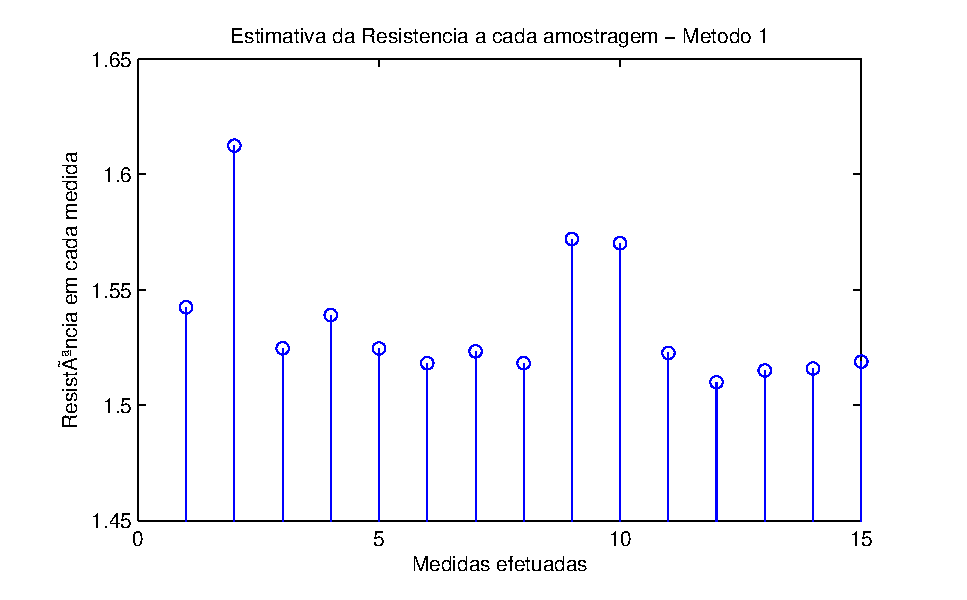
\includegraphics[width=0.98\columnwidth]{figures/method1.eps}
	\caption{Gr�fico da estimativa da resist�ncia em cada instante para o conjunto de dados da 
	primeira amostragem.}
	\label{fig:method1}
\end{figure}

Para o segundo conjunto de dados a resist�ncia estimada foi de $1567.9 \Omega$ com um desvio padr�o de
$66.7 \Omega$. Na Figura (\ref{fig:method1_b}) apresenta-se os valores estimados da resist�ncia
a cada medida.

\begin{figure}[htbp]
	\center
	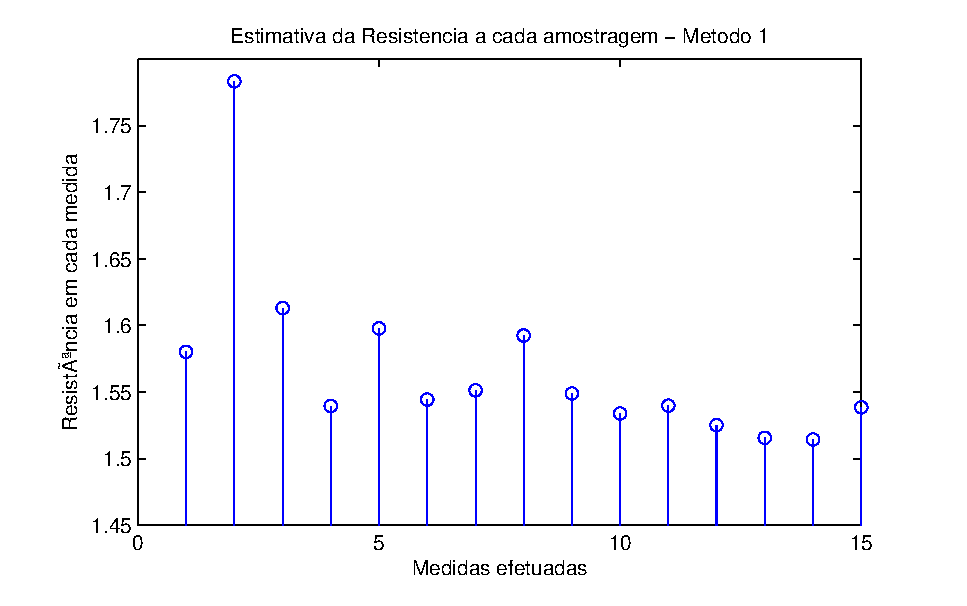
\includegraphics[width=0.98\columnwidth]{figures/method1_b.eps}
	\caption{Gr�fico da estimativa da resist�ncia em cada instante para o conjunto de dados da 
	segunda amostragem.}
	\label{fig:method1_b}
\end{figure}

Alterando-se o m�todo para a estimativa da resist�ncia para a apresentada em (\ref{eq:method2}), 
Obt�m-se uma resist�ncia de $1530.6 \Omega$.

\begin{equation}
\hat{R_2}=\frac{1}{N}\frac{\sum_{t=1}^{N}y(t)}{\sum_{t=1}^{N}u(t)}
\label{eq:method2}
\end{equation}

Para o terceiro m�todo (\ref{eq:method3}), tamb�m conhecido como m�todo dos m�nimos quadrados, 
chegou-se aos valores de resist�ncia de $ 1527.7 \Omega$ e $1538.0 \Omega$ nos conjuntos de
dados, 1 e 2 respectivamente.

\begin{equation}
\hat{R_3}=\frac{1}{N}\frac{\sum_{t=1}^{N}y^2(t)}{\sum_{t=1}^{N}u(t)y(t)}
\label{eq:method3}
\end{equation}

Observa-se que o valor estimado para a resist�ncia utilizando o m�todo dos m�nimos quadrados
obt�m valores para a resist�ncia dos conjuntos de dados 1 e 2 mais pr�ximos que quando utilizamos 
o m�todo 1.


%===============================================================================
\subsection{Compara��o dos resultados obtidos}
\label{sec:compar}

Na Tabela (\ref{tab:compar}) apresenta-se os valores de resist�ncia obtidos utilizando 
os 3 m�todos e os dois conjuntos de dados.

\begin{table}[htbp]
  \begin{center}
	\caption{Comparativo dos resultados obtidos}
	\label{tab:compar}
	\begin{small}
	  \begin{tabular}{clll}
		\hline
		Dados &  M�todo 1 & M�todo 2 & M�todo 3 \\
		\hline
		Conjunto 1 & 1535.3 & 1530.6 & 1527.7 \\
		Conjunto 2 & 1567.9	& 1547.5 & 1538.0 \\
		Conjunto 3 & 1564.0	& 1550.2 & 1545.7 \\
		\hline
		M�dia      & 1555.7 & 1542.7 & 1537.2 \\
		Desv Padr�o & 17.8  & 10.6   & 9.0    \\
		\hline
	  \end{tabular}
	\end{small}
  \end{center}
\end{table}

A partir da Tabela (\ref{tab:compar}) � poss�vel observar que dentro dos tr�s m�todos, o que 
apresentou um valor para a resist�ncia com o menor desvio padr�o entre as amostras coletadas 
foi o m�todo 3 (m�nimos quadrados).

\section{M�todo dos m�nimos quadrados}
\label{sec:mmq}
%===============================================================================

O m�todo dos m�nimos quadrados (MMQ) � um dos mais conhecidos e mais utilizados 
nas mais diversas �reas da ci�ncia e tecnologia. A origem da ideia b�sica pode ser
encontrada nos trabalhos de Gaus sobre o estudo astron�micos. \cite{aguirre}

\subsection{Sistema com solu��o �nica}
%===============================================================================

Considerando-se que o sistema que ser� observado seja linear e invariante no tempo.
Se a fun��o $f$ que descreve o sistema for n�o linear o sistema poder� em principio 
ser identificado por modelos n�o lineares. Com base nestas restri��es temos que:

\begin{equation}
\begin{matrix}
\begin{matrix}
\begin{bmatrix}
y_1\\ 
y_2\\ 
\vdots \\ 
y_n
\end{bmatrix} = &
\begin{bmatrix}
x_1 & x_2 & \cdots  & x_n
\end{bmatrix} &
\begin{bmatrix}
\theta_1\\ 
\theta_2\\ 
\vdots \\ 
\theta_n
\end{bmatrix}
\end{matrix}
\\ \\
y=X\theta
\end{matrix}
\nonumber
\end{equation}

Com $X \in \Re^{nxn}$. Desde que $X$ seja n�o singular � poss�vel determinar $\theta$:

\begin{equation}
\theta=X^{-1}y
\label{eq:mmq_base}
\end{equation}

\subsection{Sistema sobredeterminado}
%===============================================================================

Para sistemas sobredeterminados onde $ N > n$, A vari�vel $X$ da equa��o (\ref{eq:mmq_base}) fica
$X \in \Re^{Nxn}$. Como esta matriz n�o � quadrada, n�o � poss�vel de ser invertida. Multiplicando-se
a equa��o (\ref{eq:mmq_base}) por $X^T$ tem-se: \cite{aguirre}

\begin{equation}
X^Ty=X^TX\theta
\nonumber
\end{equation}

De onde vem:

\begin{equation}
\theta = [X^T X]^{-1} X^T y
\label{eq:mmq}
\end{equation}

O m�todo dos m�nimos quadrados minimiza o crit�rio apresentado em (\ref{eq:mmq_j}).

\begin{equation}
J(\theta)=\frac{1}{2N}\sum_{t=1}^{N}[y(t)-\hat{y}(t, \theta)]^2
\label{eq:mmq_j}
\end{equation}

Onde $\hat{y}(t, \theta)$ � a predi��o do sistema e pode ser representado como abaixo:

\begin{equation}
\hat{y}(t, \theta)=\theta^T \phi(t)
\nonumber
\end{equation}

Desta forma pode se dizer que o sistema real � o pr�prio sistema estimado mais algum 
erro de estimativa:

\begin{equation}
y(t) = \hat{y}(t, \theta) +e(t)=\theta^T \phi(t) + e(t)
\nonumber
\end{equation}

\subsection{Estruturas de modelagem}
%===============================================================================

De forma gen�rica modelos para descri��o de sistemas podem ser representados como em 
(\ref{eq:mmq_generic_model}).

\begin{equation}
A(q, \theta)Y(t)=\frac{B(q, \theta)}{F(q, \theta)}U(t)+\frac{C(q, \theta)}{D(q, \theta)}e(t)
\label{eq:mmq_generic_model}
\end{equation}

Onde:

\begin{equation}
\begin{matrix}
A(q, \theta)=1+a_1 q^{-1}+a_2 q^{-2}+\cdots +a_{na} q^{-na}\\
B(q, \theta)=b_1 q^{-1}+b_2 q^{-2}+\cdots +b_{nb} q^{-nb}\\ 
C(q, \theta)=1+c_1 q^{-1}+c_2 q^{-2}+\cdots +c_{nc} q^{-nc}\\ 
D(q, \theta)=1+d_1 q^{-1}+d_2 q^{-2}+\cdots +d_{na} q^{-nd}\\ 
F(q, \theta)=1+f_1 q^{-1}+f_2 q^{-2}+\cdots +f_{nf} q^{-nf} 
\end{matrix}
\nonumber
\end{equation}

Baseado nestas informa��es existem modelos onde apenas alguns destes polin�mios s�o 
diferentes de 1. Na Tabela (\ref{tab:model}) s�o apresentados alguns destes modelos
mais comumente utilizados.

\begin{table}[htbp]
  \begin{center}
	\caption{Modelos comumente utilizados para identifica��o de sistemas}
	\label{tab:model}
	\begin{small}
	  \begin{tabular}{rc}
		\hline
		Modelo & Polin�mios diferentes de 1 \\
		\hline
		FIR	& B \\
		ARX	& A B \\
		ARMAX & A B C \\
		ARMA & A C \\
		ARARMAX & A B C D \\
		OE & B F \\
		BJ & B F C D \\
		\hline
	  \end{tabular}
	\end{small}
  \end{center}
\end{table}

O m�todo dos m�nimos quadrados utiliza intrinsecamente o modelo ARX para descrever 
o modelo do sistema.

\subsection{Controle de posi��o angular do motor DC}
%===============================================================================

O sistema descrito na se��o (\ref{sec:modelling}) quando utilizamos o m�todo dos 
m�nimos quadrados, intrinsecamente utilizamos o modelo ARX (\ref{eq:mmq_arx}) para 
descrever este sistema. A partir de (\ref{eq:mmq_generic_model}) tem-se que o
modelo ARX fica (\ref{eq:mmq_arx}).

\begin{equation}
A(q, \theta)Y(t)=B(q, \theta)U(t)+e(t)
\label{eq:mmq_arx}
\end{equation}

A equa��o (\ref{eq:mmq_arx}) pode ser reescrita :

\begin{equation}
\begin{matrix}
Y(t)=b_1 q^{-1}U(t)+b_2 q^{-2}U(t)+\cdots +b_{nb} q^{-nb}U(t)\\
	 -a_1 q^{-1}Y(t)-b_2 q^{-2}Y(t)-\cdots -a_{na} q^{-na}Y(t) + e(t)
\end{matrix}
\nonumber
\end{equation}

O que pode ser escrito como em (\ref{eq:mmq_yt}).

\begin{equation}
Y(t)=\varphi ' \theta +e(t)
\label{eq:mmq_yt}
\end{equation}

Onde:

\begin{equation}
\begin{matrix}
\theta = \begin{bmatrix}
a_1\\ 
\vdots \\ 
a_{na}\\ 
b_1\\ 
\vdots \\ 
b_{nb}
\end{bmatrix}
 & 
\varphi (t)=\begin{bmatrix}
y(t-1)\\ 
\vdots \\ 
y(t-na)\\ 
u(t-1)\\ 
\vdots \\ 
u(t-nb)
\end{bmatrix}
\\ 
& \\
\Phi = \begin{bmatrix}
\varphi '(1)\\ 
\varphi '(2)\\ 
\vdots\\ 
\varphi '(N)
\end{bmatrix} & 
\end{matrix}
\nonumber
\end{equation}

Para o sistema de posicionamento do motor DC, a equa��o (\ref{eq:mmq_arx})
fica como em (\ref{eq:mmq_motor_arx}).

\begin{equation}
G(q, \theta)=\frac{a}{(q-b)(q-c)} \;\;H(q, \theta)=\frac{q^2}{(q-b)(q-c)}
\label{eq:mmq_motor_arx}
\end{equation}

A partir de (\ref{eq:mmq_motor_arx}) tem-se que o modelo pode ser descrito como 
abaixo:

\begin{equation}
\begin{matrix}
\theta = \begin{bmatrix}
a & b+c & c
\end{bmatrix}
&
\varphi (t)=\begin{bmatrix}
r(t-2)\\ 
y(t-1)\\ 
y(t-2)
\end{bmatrix}
\end{matrix}
\nonumber
\end{equation}

Sabe-se de antem�o que o valor esperado para a vari�vel $c$ � zero, j� que existe um 
integrador na planta em estudo. No Ap�ndice (\ref{appendix_mmq}) est� o script utilizado 
para chegar-se aos resultados obtidos para a estimativa do modelo utilizando o m�todo dos
m�nimos quadrados.

A figura (\ref{fig:mmq_arx}) apresenta os resultados obtidos na estimativa dos par�metros
a partir das medidas efetuadas sobre o sistema.

\begin{figure}[htbp]
	\center
	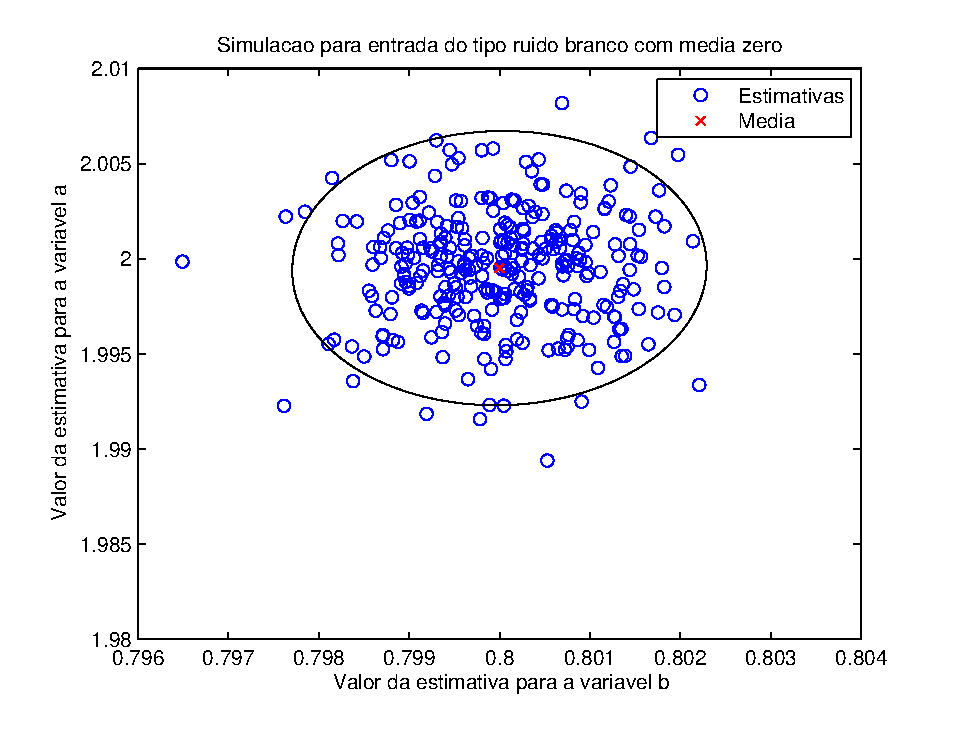
\includegraphics[width=0.98\columnwidth]{figures/mmq_arx.eps}
	\caption{TODO}
	\label{fig:mmq_arx}
\end{figure}

TODO: colocar os valores m�dios obtidos para os par�metros.

\subsubsection{Resultados para um modelo incompleto}
%===============================================================================

Nesta se��o ser� apresentado resultados para uma estimativa utilizando um modelo que n�o consegue
descrever o sistema propriamente. Ser�o utilizados os mesmos dados da estimativa do item anterior.

O modelo utilizado � descrito em (\ref{eq:mmq_motor_arx_inc}). Observa-se que o integrador n�o esta presente
neste modelo, desta forma tem-se que o modelo das vari�veis a serem utilizadas no m�todo dos 
m�nimos quadrados fica como em (\ref{eq:mmq_arx_inc_var}).

\begin{equation}
G(q, \theta)=\frac{a}{(q-b)} \;\;H(q, \theta)=\frac{q}{(q-b)}
\label{eq:mmq_motor_arx_inc}
\end{equation}

\begin{equation}
\begin{matrix}
\theta = \begin{bmatrix}
a & b 
\end{bmatrix}
&
\varphi (t)=\begin{bmatrix}
r(t-1)\\ 
y(t-1) 
\end{bmatrix}
\end{matrix}
\label{eq:mmq_arx_inc_var}
\end{equation}

Para este modelo chegou-se aos valores dos par�metros $a$ e $b$ apresentados na 
Figura (\ref{fig:mmq_arx_inc}).

\begin{figure}[htbp]
	\center
	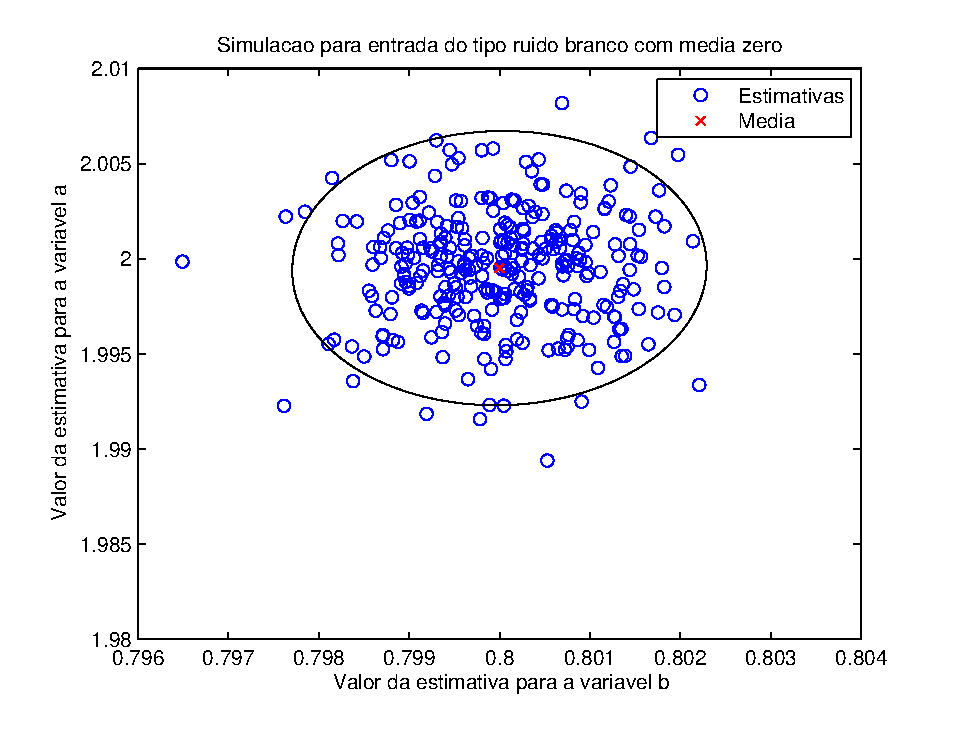
\includegraphics[width=0.98\columnwidth]{figures/mmq_arx.eps}
	\caption{TODO}
	\label{fig:mmq_arx_inc}
\end{figure}


%===============================================================================
\section{Conclus�es}
\label{sec:concl}
%===============================================================================

Neste trabalho foram apresentados dois m�todos para identifica��o de sistemas lineares,
ambos os m�todos se encontram na categoria de m�todos param�tricos de identifica��o, que 
de forma simplificada, tentam estimar os par�metros de uma fun��o de transfer�ncia que
represente o sistema f�sico em quest�o. Os m�todos utilizados foram o dos m�nimos quadrados
e das vari�veis instrumentais.

O sistema f�sico utilizado foi o controle de posi��o de um motor DC, e os dados coletados
para a identifica��o foram gerados a partir da aplica��o de sinais de refer�ncia tais como
rampas, senoides e ondas quadradas. Para cada um destes conjuntos foi obtido uma estimativa
dos par�metros do modelo utilizado.

Para efetuar a estimativa do sistema f�sico em quest�o, foi necess�rio determinar um modelo,
este foi determinado baseado no conhecimento das caracter�sticas do sistema e algumas simplifica��es 
foram efetuadas, a fim de tornar o modelo matem�tico o mais simples poss�vel, mas que ainda 
consiga descrever o sistema dentro de uma margem aceit�vel de precis�o.

O m�todo dos m�nimos quadrados (\ref{sec:mmq}) obteve resultados para a estimativa dos par�metros
que podem ser encontrados na Tabela (\ref{tab:mmq_results}). Houveram pequenas diverg�ncias nos 
par�metros entre um conjunto de dados e outro, o que n�o � desej�vel, isso pode ser devido a
imprecis�es do modelo utilizado, (pode ser devido as simplifica��es do modelo, ou de din�micas n�o
levadas em considera��o).

O m�todo das vari�veis instrumentais (\ref{sec:iv}) obteve resultados semelhantes ao m�todo 
dos m�nimos quadrados, mas com valores mais pr�ximos nos diferentes grupos de medidas. Os 
resultados para este m�todo foram apresentados na Tabela (\ref{tab:iv_results}).

De forma geral este trabalho abordou e demonstrou como � o procedimento e no que se baseiam 
dois m�todos de identifica��o de sistemas lineares sujeitos a incertezas, perturba��es e 
ru�dos. N�o � o objetivo deste trabalho detalhar esmiu�ar a matem�tica destes m�todos e
sim apresentar um exemplo pr�tico, e demonstrar sua utilidade.

A aplicabilidade deste t�pico de engenharia � de uma aplicabilidade imensa, sendo muito importante 
nas mais diversas �reas a correta identifica��o de sistemas para que, a partir do conhecimento 
matem�tico de sua din�mica, possa se agir sobre este sistema, a fim de obter os resultados desejados
de forma eficiente e com propriedade sobre as a��es tomadas, uma vez que o sistema identificado
� identificado e sabe-se o qu�o boa esta aproxima��o do sistema real pode ser.

%===============================================================================
\appendix
%===============================================================================
\chapter{1 - Script para Simula��o do MQ para o modelo ARX} 
\label{appendix_mmq}
\lstset{caption=M�todo dos m�nimos quadrados,label=DescriptiveLabel}
\lstinputlisting{matlab_files/simul.m}

%===============================================================================
\chapter{2 - Script para Simula��o do m�todo das vari�veis instrumentais} 
\label{appendix_iv}
\lstset{caption=M�todo das vari�veis instrumentais,label=DescriptiveLabel}
\lstinputlisting{matlab_files/simul_iv.m}

%===============================================================================



\bibliographystyle{IEEEtran}
\bibliography{biblio}

\end{document}
